\chapter{Week 12 -- Data-Driven Methods}

\section{Abstract}
This report presents results of an experiment with data-driven methods and their use in battery modelling and prediction tasks. Using a dataset of 380 charging and discharging cycles from accelerated cell aging, a Random Forest regressor is trained to predict the remaining capacity of the cell (essentially predicting the SOH-C) using only a few pieces of information (features) from the full charging cycle.

\section{Familiarization with the environment}

In contrast to previous lab reports relying heavily on Matlab live scripts, this one was prepared using python in the Jupyer notebook environment. All tasks are performed on a dataset from the University of Michigan\footnote{available at \url{https://deepblue.lib.umich.edu/data/downloads/gq67jr501}}. It contains measurements such as cell voltage, current or temperature from 380 full battery cycles periodically sampled every 10 seconds. Since the task only deals with charging half-cycles, all time instants with current $i < \SI{0}{\ampere}$ are removed from the working dataset.

Most of the processing was done using the python library \texttt{pandas}. It provides means of loading the dataset using \texttt{pd.read\_csv}, accessing individual signals using \texttt{dataset[signal\_name]} and performing logical indexing (slicing) by \texttt{dataset[boolean\_mask]}. This is especially useful for operations such as extracting a particular full cycle or detecting discharging instants. Additionally, \texttt{matplotlib.pyplot} was used for visualization of signals.

The learning part of this lab was performed using the popular python package \texttt{scikit-learn}. It provides interface to many machine learning constructs such as metrics (loss functions, e.g. \texttt{mean\_squared\_error}), utilities such as \texttt{train\_test\_split} for simple creation of evaluation datasets for cross-validation, or the actual trainable models, such as the ensemble model \texttt{RandomForestRegressor} used in this task. 

\begin{figure}
\centering
\begin{minipage}{0.49\textwidth}
    \centering
    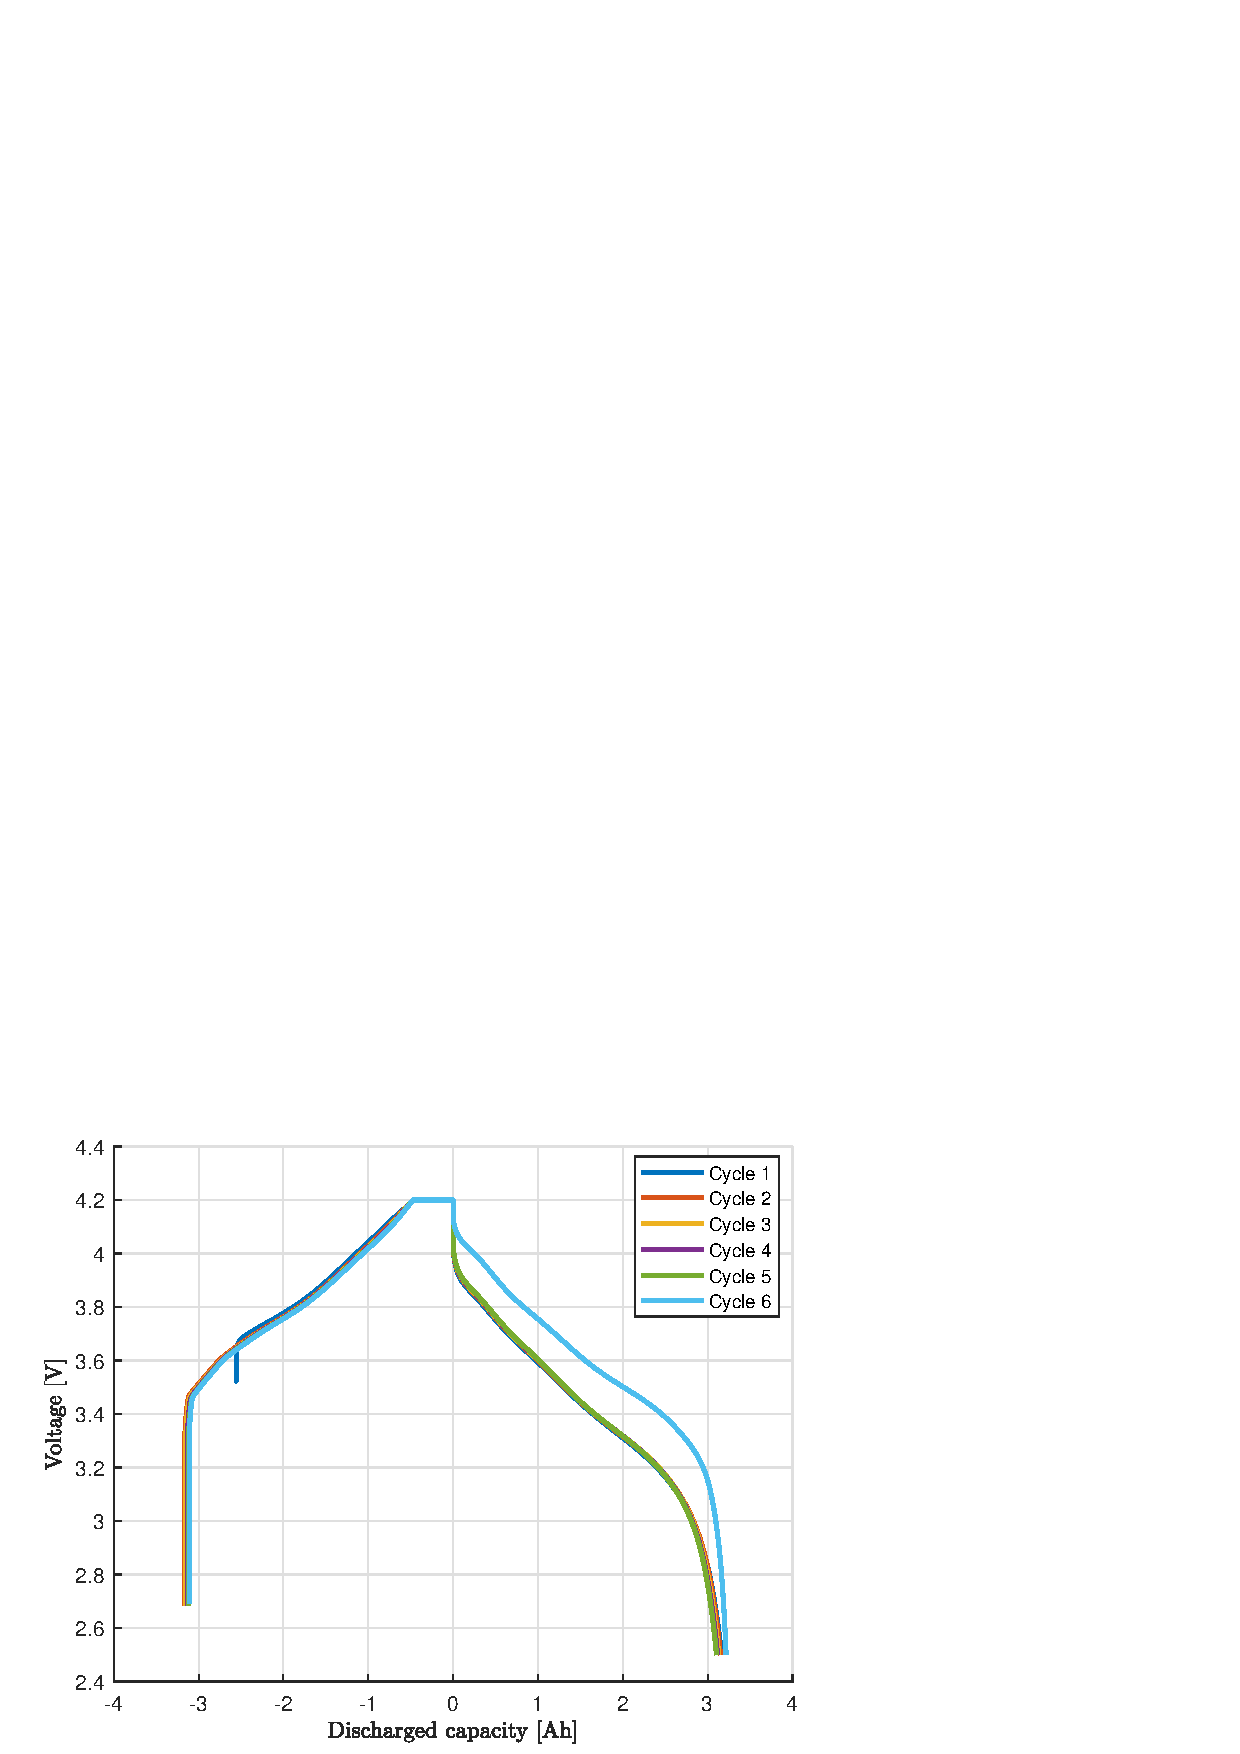
\includegraphics[width=\linewidth]{figures/12/voltages.jpg}
    \caption{Voltages during several full battery cycles.}
    \label{fig:12-voltages}
\end{minipage}
\hfill
\begin{minipage}{0.49\textwidth}
    \centering
    \includegraphics[width=\linewidth]{figures/12/currents.jpg}
    \caption{Currents during several full battery cycles.}
    \label{fig:12-currents}
\end{minipage}
\end{figure}

\section{Training the regressor}

To verify that the provided dataset can be used for the training of an SOH-C predictor, one can plot and analyze measurements from several cycles. Fig. \ref{fig:12-voltages} through \ref{fig:12-capacities} show the recorded cell voltage, flowing current and capacity, respectively. The charging mode is clearly CC-CV with current limit of 1000 mA and target voltage of 4.2 V. It is apparent from all figures/12 that with a growing number of elapsed cycles, the cell ages and loses capacity, making subsequent cycles shorter (the voltage in Fig. \ref{fig:12-voltages} rises faster and the current in \ref{fig:12-currents} drops earlier). 
Additionally, the total capacity gradually decreases, as shown in Fig. \ref{fig:12-aging}. There are several outlier cycles that were interrupted early for unspecified reasons.

Out of the total of 380 recorded cycles, 19 were randomly selected for final testing. The rest was divided into the training and validation dataset according to the 80:20 Pareto rule. Instead of using all collected samples (roughly 2000 of them per signal per cycle) as inputs to the machine learning algorithm, information from each cycle is condensed into a small vector of features. The Random Forrest is an ensemble algorithm for supervised learning that separately trains many decision trees on subsets of the training data and then combines (e.g. averages) their outputs when asked to predict the output for previously unseen data. In this task, the number of trees in the forest (an algorithm hyperparameter) was chosen as 100.

\begin{figure}
\centering
\begin{minipage}{0.49\textwidth}
    \centering
    \includegraphics[width=\linewidth]{figures/12/capacities.jpg}
    \caption{Cell capacity during several full battery cycles.}
    \label{fig:12-capacities}
\end{minipage}
\hfill
\begin{minipage}{0.49\textwidth}
    \centering
    \includegraphics[width=\linewidth]{figures/12/aging.jpg}
    \caption{The loss of total cell capacity due to aging.}
    \label{fig:12-aging}
\end{minipage}
\end{figure}

\subsection{Selection of features}

The best performance (the lowest error on the test set) was achieved using the features listed in Table \ref{tab:12-importance} in the decreasing order of mean importance. Said simply\footnote{More detailed explanation of the feature importance can be found at \url{https://medium.com/the-artificial-impostor/feature-importance-measures-for-tree-models-part-i-47f187c1a2c3} and in resources linked there.}, the \textit{Mean Decrease in Impurity (MDI)} used by \texttt{scikit} measures the importance of a feature as the number of decision nodes that branch paths based on said feature weighted by the probability of reaching said nodes. 
High feature importance means that many decision tree nodes are branching the path based on said feature and that they reside in busy subtrees of the whole tree hit by many input samples.
On the other hand, negligible feature importance shows that the tree did not need to incorporate said feature into its decision nodes during training. Since this metric is calculated for each tree separately, the third column of Table \ref{tab:12-importance} shows the standard deviation of importances across the whole forest. Note that many of these standard deviations are quite significant, hinting that indeed each tree puts emphasis on entirely different features.

\begin{table}[]
    \centering
    \begin{tabular}{c|c|c}
    Feature name & Mean importance & Standard deviation of importance \\ \hline
Temperature Delta & 0.4250 & 0.3142 \\
Number of Samples & 0.3646 & 0.2996 \\
Total Charge   & 0.1022 & 0.1987 \\
Average Current & 0.0411 & 0.1223 \\
Maximal V      & 0.0360 & 0.1129 \\
Current Standard Deviation & 0.0216 & 0.0830 \\
Average Temperature & 0.0048 & 0.0329 \\
Minimal V      & 0.0047 & 0.0333 \\
    \end{tabular}
    \caption{Importance of individual features for individual trees in the ensemble model}
    \label{tab:12-importance}
\end{table}

The presence of the number of samples collected during the charging cycle among the most important features is expected, as it indirectly expresses the duration of charging half-cycle and that is significantly influenced by the cell's capacity when using CC-CV scheme, as shown e.g. in Fig. \ref{fig:12-currents}. However what is not expected at all is the high importance of the temperature delta. In order to explain it, measurements of the cell's internal resistance available in the dataset have to be used. The evolution of the real part of cell's impedance as a function of the available capacity over the course of the experiment is shown in Fig. \ref{fig:12-R}. The ohmic resistance clearly grows (yet again proving that the dataset indeed describes a noticeably aging cell, in this case with respect to SOH-R), causing increased losses due to constant charging current, eventually resulting in greater temperature delta.

Some features on the other hand were identified by the algorithm as mostly irrelevant, e.g. the minimal and maximal voltage. This can be explained intuitively as well - all charging half-cycles end at 4.2 V (giving no useful information about the cell capacity) and the starting voltage is subject to slight unpredictable variation caused by transition from one cycle to the next.

\begin{figure}
    \centering
    \includegraphics[width=0.5\linewidth]{figures/12/R.jpg}
    \caption{Real part of the cell impedance during ageing}
    \label{fig:12-R}
\end{figure}

\subsection{Evaluation of the Regressor}

The model's performance after training was evaluated using the test set. True cell capacities and the corresponding model predictions are shown in Fig. \ref{fig:12-pred}. The histogram of prediction errors shown in Fig. \ref{fig:12-pred-error-hist} suggests that the model tends to underestimate the true capacity slightly (by less than 15 mAh) with the exception of two outliers with grater prediction error.
The algorithm's performance was assessed using several metrics listed in Table \ref{tab:12-test-error}. Their values are derived from the prediction error expressed in Ah, i.e. the greatest single prediction error was 22.9 mAh and the average prediction error was 6.93 mAh.

\begin{table}[]
    \centering
    \begin{tabular}{c|c}
        Error metric & Magnitude \\\hline
        Maximal error                  & 2.29e-02 \\
        Mean Absolute Deviation (MAD)  & 6.93e-03 \\
        Mean squared error (MSE)       & 8.35e-05 \\
    \end{tabular}
    \caption{Prediction error achieved on the test set}
    \label{tab:12-test-error}
\end{table}




\begin{figure}
\centering
\begin{minipage}{0.49\textwidth}
    \centering
    \includegraphics[width=\linewidth]{figures/12/test.jpg}
    \caption{Regressor performance on the test set.}
    \label{fig:12-pred}
\end{minipage}
\hfill
\begin{minipage}{0.49\textwidth}
    \centering
    \includegraphics[width=\linewidth]{figures/12/pred-error-hist.jpg}
    \caption{Capacity prediction error on the test set.}
    \label{fig:12-pred-error-hist}
\end{minipage}
\end{figure}


